\documentclass[letterpaper, 10 pt, conference]{ieeeconf}\IEEEoverridecommandlockouts%\overrideIEEEmargins
\usepackage[dvips]{epsfig}
\usepackage{amsmath}
\usepackage{cite}
\usepackage[psamsfonts]{amssymb}
\usepackage{dsfont}
\usepackage{multirow}
\usepackage[ruled,vlined,commentsnumbered]{algorithm2e}
\usepackage{caption}


\renewcommand\arraystretch{1.5}

\newtheorem{theorem}{Theorem}
\newtheorem{assumption}{Assumption}
\newtheorem{proposition}{Proposition}
\newtheorem{lemma}{Lemma}
\newtheorem{remark}{Remark}

\topmargin -0.3in
%%%%%%%%%%%%%%%%%%%%%%%%%%%%%%%%%%%%%%%%%%%%%%%%%%%%%%%%%%%%%%%%%%%%%%%%%%%%%%%%%%%%%%%%%%%%%%%%%%%%%%%%%%%%%%%%%%%%%%%%%%%%%%%%%%%%%%%%%%%%%%%%%%%%%%%%%

\title{\LARGE \bf Optimization-Based Event-Triggered Predictive Control of Process Systems with Control and Communication Constraints}

\author{Da Xue and Nael H. El-Farra$^{\dag}$\thanks{$^{\dag}$ To whom correspondence should be addressed:
{\tt E-mail: nhelfarra@ucdavis.edu}. Financial support by NSF, CBET-1438456, is gratefully acknowledged.} \\
Department of Chemical Engineering\\
University of California, Davis, CA 95616 USA}

\begin{document}
\newcommand{\bx}{\mathbf{x}}
\newcommand{\bxh}{\widehat{\mathbf{x}}}
\newcommand{\be}{\mathbf{e}}
\newcommand{\bu}{\mathbf{u}}
\newcommand{\bA}{\mathbf{A}}
\newcommand{\bK}{\mathbf{K}}
\newcommand{\bAh}{\widehat{\mathbf{A}}}
\newcommand{\bB}{\mathbf{B}}
\newcommand{\bBh}{\widehat{\mathbf{B}}}
\newcommand{\Rs}{{\rm I}\!{\rm R}}
\newcommand{\dis}{\displaystyle}
\newcommand{\Rset}{{\rm I}\!{\rm R}}
\newcommand{\ovl}{\overline}
\newcommand{\unl}{\underline}
\newcommand{\ovb}{\overbrace}
\newcommand{\td}{\tilde}
\newcommand{\norm}[1]{\|\,#1\,\|}

\renewcommand{\thefootnote}{\fnsymbol{footnote}}

%\bibliographystyle{IEEEtran}

\maketitle \thispagestyle{empty} \pagestyle{empty}

\begin{abstract}

This work presents an optimization-based controller design methodology for networked control systems subject to uncertain dynamics and sensor-controller communication constraints. The proposed methodology aims to enforce desired closed-loop stability and performance properties while minimizing communication cost at the same time. Initially, an auxiliary model-based state-feedback controller is designed, and the relationship between controller gain and the maximum allowable model-update period that ensures closed-loop stability under periodic sensor-controller communication is characterized. A cost function that explicitly penalizes on system performance, control action as well as minimum allowable communication frequency (inverse of the maximum allowable model-update period) is then formulated. By solving the unconstrained optimization problem in a receding horizon fashion, the optimal controller gain and the maximum allowable model-update period can be determined simultaneously. The controller is implementated only for the first update period. At the end of the model update period, real-time measurement is sampled and transmitted to update the model state, and the optimization problem is solved again. The results are illustrated using simulation examples.

\end{abstract}

%%%%%%%%%%%%%%%%%%%%%%%%%%%%%%%%%%%%%%%%%%%%%%%%%%%%%%%%%%%%%%%%%%%%%%%%%%%%%%%%%%%%%%%%%%%%%%%%%%%%%%%%%%%%%%%%%%%%%%%%%%%%%%%%%%%%%%%%%%%%%%%%%%%%%%%%%

\section{Introduction}

The design and analysis of networked control systems have been the subject of significant research interest over the last two decades, both in the industrial and academic circles (e.g., see \cite{hespanha2007survey,gupta2010networked,ke2013survey} for surveys of results in this area). The operational flexibility and substantial economic savings realized through networked control architectures have been a major driving force behind the increased reliance in industrial practice on sensor and control systems that are accessed over shared communication networks. The integration of wireless sensor networks in process control systems, for example, is an appealing goal that promises to expand the capabilities of existing control technology beyond what is possible with wired devices alone, and is regarded as a key enabling mechanism for the transition towards smart plant operations \cite{christofides2007smart}. At the same time, the various fundamental challenges introduced by this technology from a control point of view have motivated numerous research studies. One of the key challenges is the development of resource-aware control methods that can systematically balance the desired stability and performance requirements against the intrinsic constraints on the sensing, computation and communication resources of the networked devices as well as the occasional unreliability of the communication medium due to interference in the field or environmental impact. On the one hand, maximizing control system performance often requires frequent sensor-controller communication and increased levels of network resource utilization. Reducing communication costs, on the other hand, favors keeping the sensing and communication levels to a minimum which can lead to reduced control system performance.

To balance desired closed-loop performance and communication cost, a quasi-decentralized model-based networked control structure that enforces closed-loop stability with minimal periodic communication was developed in \cite{sun2008quasi}. The key idea was to embed a set of predictive models to generate control actions during communication intervals when state measurement is not accessible to the controller, and to update the model state when communication is restored at periodic model update time. The maximum allowable model update period can be explicitly characterized to achieve closed-loop stability and facilitate the time-triggered communication policy. 


An alternative approach for dealing with communication constraints in networked control systems is the use of event-triggered control strategies which has been widely studied. In these strategies, sensor-controller communication over the network is typically suspended or restored in response to certain events which are tied to some specified closed-loop stability and/or performance thresholds. The aim is to keep network utilization to a minimum while guaranteeing minimal levels of control performance. The approach typically starts with the design of a model-based stabilizing feedback controller and ends with the derivation of a constant or state-dependent stability threshold which is used as a trigger for sensor-controller communication. The implementation generally involves monitoring the model estimation error during periods of communication suspension and updating the model states in the event that the stability threshold is breached. Among these studies, \cite{moreira2016event,groff2016observer} formulate optimization problems to tune the update trigger functions aiming at further reducing network utilization. This approach of event-triggered control is appealing in the context of sensor/actuator networks where reducing network utilization can also reduce the energy expenditures of battery powered wireless devices, and has been widely studied in recent years (e.g., see \cite{mazo2011decentralized,wang2011event,garcia2013model,xue2016actuator} for some results in this area). 

The appealing features of this approach notwithstanding, a close examination of existing event-triggered control strategies reveals a general lack of explicit control performance optimization in the controller design methodology. In the context of balancing the intrinsic tradeoff between control performance and network resource utilization, there is an apparent increased emphasis on reducing network utilization, often at the expense of control system performance. %In addition to the lack of performance optimization considerations, practical implementation considerations such as the presence of constraints on the state and manipulated variables, which are commonly encountered in practical applications, are also ignored in the design formulation. These considerations not only limit the achievable control quality but can also lead to closed-loop instability if not explicitly accounted for at the controller design stage.

Motivated by these considerations, we present in this work an optimization-based controller and communication design methodology for systems subject to state, control and sensor-controller communication constraints. The objective is to optimize the control system performance while minimizing communication costs and network utilization at the same time. To this end, an auxiliary model-based state-feedback controller is initially designed and used to obtain the minimum allowable model update frequency for closed-loop stability as if periodic communication was to be used. A finite-horizon unconstrained optimal control problem in which the objective function includes explicit penalties on the states, the control action and the model udpate frequency is then formulated. The optimization problem is solved in a receding horizon fashion to obtain the optimal controller design parameters over the horizon. Unlike conventional model predictive control formulations, however, the optimization problem is re-solved and the model states are updated at the model update time. Because of the special formulation of the optimization problem, the optimal controller is not only designed to reduce network utilization, but to balance performance requirements and communication cost associated. Its capability of dynamically coordinating control action and communication to irregular operation conditions, or robustness to disturbances, is another appealing feature. Finally, the developed methodology is tested and illustrated using a numerical example and a siimulated chemical process example.

%%%%%%%%%%%%%%%%%%%%%%%%%%%%%%%%%%%%%%%%%%%%%%%%%%%%%%%%%%%%%%%%%%%%%%%%%%%%%%%%%%%%%%%%%%%%%%%%%%%%%%%%%%%%%%%%%%%%%%%%%%%%%%%%%%%%%%%%%%%%%%%%%%%%%%%%%

\section{Preliminaries}\label{sec:preliminaries}
\subsection{Class of systems}
We consider continuous-time linear systems with the following state-space representation:
\begin{equation}\label{eqn:PlantState}
  \dot{\bx} = \bA\bx + \bB\bu
\end{equation}
where $\bx\in\mathbb{R}^{n_{\bx}}$ is the vector of the state variables, $\bu\in\mathbb{R}^{n_{\bu}}$ is the vector of manipulated inputs, $\bA$ and $\bB$ are constant matrices. Without loss of generality, the origin is assume to be an equilibrium point of the uncontrolled system.

%%%%%%%%%%%%%%%%%%%%%%%%%%%%%%%%%%%%%%%%%%%%%%%%%%%%%%%%%%%%%%%%%%%%%%%%%%%%%%%%%%%%%%%%%%%%%%%%%%%%%%%%%%%%%%%%%%%%%%%%%%%%%%%%%%%%%%%%%%%%%%%%%%%%%%%%%

\subsection{Model-based networked control using periodic communication/sampling}\label{sec:PeriodicCommu}
We consider a typical model-based networked control structure in which an uncertain model of the system of Eq.\ref{eqn:ModelState} is included in the controller.
\begin{equation}\label{eqn:ModelState}
  \dot{\bxh} = \bAh\bxh + \bBh\bu
\end{equation}
where $\bxh\in\mathbb{R}^{n_{\bx}}$ is the vector of the model state variables, it is an estimate on the plant state $\bx$, $\bAh$ and $\bBh$ are constants matrices that approximate the matrices $\bA$ and $\bB$, respectively, in Eq.\ref{eqn:ModelState} and are given by:
\begin{equation}\label{eqn:ModelUncertainty}
  \bA = \bAh + \delta_{\bA},\ \bB = \bBh + \delta_{\bB}
\end{equation}
 We first design an auxiliary state-feedback controller of the form Eq.\ref{eqn:Controller} and investigate the maximum allowable update period if a periodic communication strategy is to be used.
\begin{equation}\label{eqn:Controller}
  \bu = \bK\bxh
\end{equation}
Refer to Yulei's paper, if the model state $\bxh$ is updated periodically with an update period $h$ such that the eigenvalues of the following test matrix
\begin{equation}\label{eqn:StabilityCondition}
  M(h) = \left[\begin{array}{cc}
          I_{m\times m} & O_{m\times m}\\
          O_{m\times m} & O_{m\times m}
        \end{array}\right]e^{h\Lambda}\left[\begin{array}{cc}
          I_{m\times m} & O_{m\times m}\\
          O_{m\times m} & O_{m\times m}
        \end{array}\right]
\end{equation}
are strictly inside the unit circle, then the overall closed-loop system is globally exponentially stable, where $m = \mathbb{R}^{n_{\bx}}$, $I_{m\times m}$ is the $m\times m$ identity matrix and $O_{m\times m}$ is the $m\times m$ zeros matrix, and
\begin{equation}
  \Lambda = \left[\begin{array}{cc}
              (\bA + \bB\bK)                    & -\bB\bK\\
              (\delta_{\bA} + \delta_{\bB}\bK)  & (\bAh - \delta_{\bB}\bK)
            \end{array}\right]
\end{equation}
This can be proved by defining the model estimation error $\be(t) = \bx(t) - \bxh(t)$. Direct substitution of Eq.\ref{eqn:PlantState} and Eq.\ref{eqn:ModelState} yields
\begin{equation}
  \dot{\be} = \dot{\bx} - \dot{\bxh} = (\delta_{\bA} + \delta_{\bB}\bK)\bx + (\bAh - \delta_{\bB}\bK)
\end{equation}
Defining the augmented state $\xi(t) = [\bx^T(t)\ \be^T(t)]^T$, we can rewrite the closed-loop dynamics of the overall plant as
\begin{equation}
  \dot{\xi} = \Lambda\xi
\end{equation}
Notice that the model state $\bxh$ is updated using real-time measurement $\bx$ at every measurement transmission time $t_k$, $k = 1,2,\cdots$,  so that$\be(t_k) = 0$, or $\xi(t_k) = [\bx^T(t_k)\ 0]^T$ $\forall k$. Therefore $\xi$ is made up of a continuous component and a discrete component. One can further prove that with the initial condition $\xi(t_0) = [\bx^T(t_0)\ 0 = \xi_0]^T$
\begin{equation}
  \xi(t) = e^{\Lambda(t - t_k)}(I_se^{\Lambda h}I_s)^k\xi_0 =  e^{\Lambda(t - t_k)}M^k\xi_0
\end{equation}
where $I_s = \dis{\left[\begin{array}{cc}
          I_{m\times m} & O_{m\times m}\\
          O_{m\times m} & O_{m\times m}
        \end{array}\right]}$. As $e^{\Lambda(t - t_k)}$ and $\xi_0$ are both finite, the eigenvalues of $M$ lying strictly within the unit circle ensures the globally exponential stability.


%%%%%%%%%%%%%%%%%%%%%%%%%%%%%%%%%%%%%%%%%%%%%%%%%%%%%%%%%%%%%%%%%%%%%%%%%%%%%%%%%%%%%%%%%%%%%%%%%%%%%%%%%%%%%%%%%%%%%%%%%%%%%%%%%%%%%%%%%%%%%%%%%%%%%%%%%
\section{Optimization-based controller design method}
Section \ref{sec:preliminaries} provides an important theory foundation for a state-feedback controller to be implemented under periodic model update. It proves that globally exponential closed-loop stability is guaranteed as long as the model state is updated periodictly with the update period being no longer than the maximum allowable update period characterized from the stability condition of Eq.\ref{eqn:StabilityCondition}. However, some earlier articles (\cite{sun2010quasi,xue2016supervisory} for example)  argued that the periodic communication is able to reduce network utilization to a minimum but is not robust to changes in operating conditions as the communication period is fixed at the controller design state and would not change during plant oerations. To overcome such limiations but still appreciate its beauty in the controller and communication design and analysis, in this section, we relax the periodic communication strategy but use its stability condition to devise an optimization-based controller and communication design methodology.


\subsection{Optimization problem formulation}
Instead of one-time determination and fixing the model update frequency at the controller design stage, in this section, we propose a dynamically coordinated deternimation of the control feedback gain and model udpate frequency using an on-line optmization method. The optimization problem is formulated as follows.
\begin{subequations}\label{eqn:Optimization}
  \begin{align}
    &\min_{K_k, h_k} J = \int_{t_k}^{t_k+H} \hspace{-4mm} [\bxh^T(t)W_x\bxh(t) + \bu^T(t)W_u\bu(t)]dt + J_c(h_k)\\
               % &= \int_{t_k}^{t_k+H} \hspace{-2mm} [\bxh^T(t)(W_x + \bK_k^TW_u\bK_k)\bxh(t)]dt + \frac{W_h}{h_k(K)}\\
    &\text{subject to:}\nonumber\\
    &\bxh(t) = \widehat{A}\bxh(t) + \widehat{B}\bu(t)\\ \label{eqn:Opt_xhat}
    &\bu(t) = K_k(\bxh(t))\\
    &\lambda_{\max}\{M(K_k, h_k)\} < 1 \label{eqn:Opt_stability}
  \end{align}
\end{subequations}
where $t_k$, $k = 1,2,\cdots$ and $H$ denote the $k^{th}$ model update time and the optimization horizon, respectively. $\bxh(t)\in\mathbb{R}^{n_{\bx}}$ denotes the state of the plant model whose dynamic is governed by Eq.\ref{eqn:Opt_xhat}. $\bu(t)$ is the control input which is a function of the model state $\bxh(t)$. In fact, the cost function $J$ can be simplified to $J = \int_{t_k}^{t_k+H}[\bxh^T(t)(W_x + K_k^TW_uK_k)\bxh(t)]dt + J_c(h_k)$. $W_x$, and $W_u$ are the positive definite weighting matrices on the closed-loop state, and the manipulated input, respectively. $J_c(h_k)$ is the non-singular communication cost function whose value depends on the decision of the communication period $h_k$. The optimization variables are the controller gain $K_k$, and the model update period $h_k$. The pair of $K_k$ and $h_k$ must satisfy the stability condition in Eq.\ref{eqn:Opt_stability}. The solution to this optimization problem finds the optimal pair of ($K_k$, $h_k$) that minimizes the cost function $J$.

For controller implementation, the optimization problem is solved on-line and the optimal controller gain $K_k$ and the corresponding stabilizing model udpate period $h_k$ is implemented in a receding horizon fashion as shown in Fig.\ref{fig:RecedingHorizon}. To be more specific, at the beginning of plant operation $t_0$, the optimization problem of Eq.\ref{eqn:Optimization} is solved and the solution $K_0$ yields the stabilizing model update period $h_0$. The controller $K_0$ is only implemented for $t \in [0,h_0)$, and by the end of the model update period, the model-based controller collects state measurements from the sensors and update the model state. With the updated model state, the optimization problem of Eq.\ref{eqn:Optimization} is solved gain to obtain $K_1$ and $h_1$ at $t = h_0$. $K_1$ is then implemented for $t \in [h_0,(h_0+h_1))$ and the optimization problem is re-solved by the end of the first model update period of the new optimization horizon. In general, at the $k^{th}$ model update, the optimization problem of Eq.\ref{eqn:Optimization} is solved over the horizon $H$, resulting in the optimal controller gain $K_k$, and model update period $h_k$. The controller $K_k$ is implemented for $t \in [t_k, (t_k+h_k))$ and model udpate is performed and the optimization problem is re-solved at the end of the first period. Algorithm 1 summarizes the controller and communication design and implementation procedures.

\begin{figure}[hptb]
  \centerline{\hspace{2mm}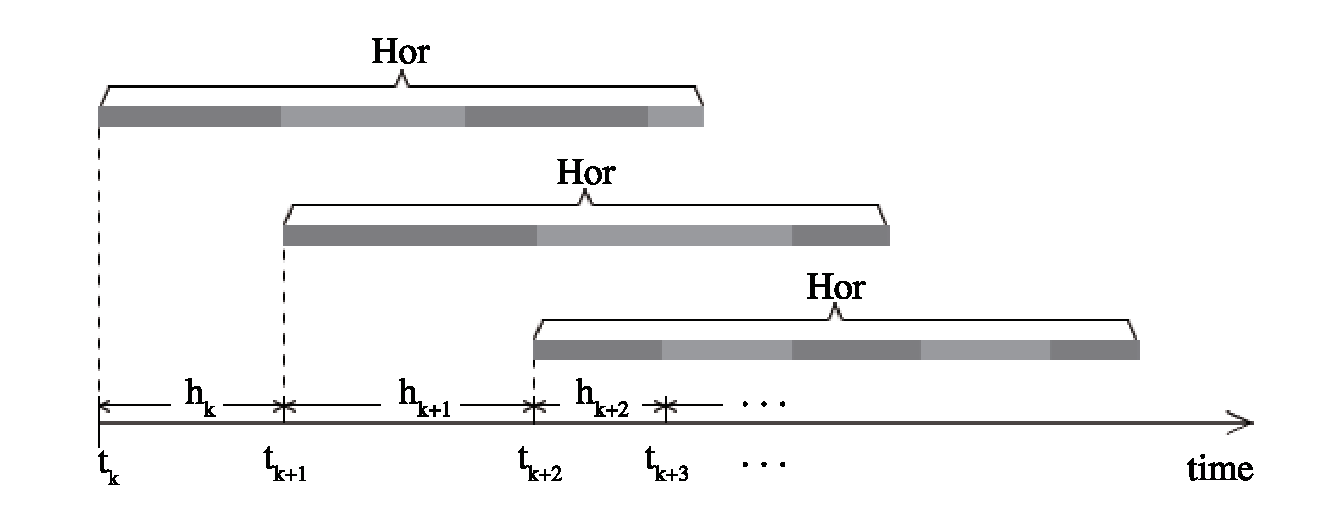
\psfig{file=RecedingHorizon.eps,height=1.25in,width=3.6in,clip=}\hspace{-4mm}{\footnotesize}}
  \caption{Receding horizon implementation of controller and communication}\label{fig:RecedingHorizon}
\end{figure}

% \subsection{Controller design and implementation algorithm}
\LinesNumbered\IncMargin{1em}
\begin{algorithm}\label{algorithm}
  \textbf{characterize} $h(K)$ from stability conditon Eq.\ref{eqn:Opt_stability}\; \label{alg:CharH}
  \textbf{input} $W_x$, $W_u$, $W_h$\;
  \textbf{initialize} $\bxh(t_0) = \bx(t_0)$\;\label{alg:init}
  \textbf{solve} Eq.\ref{eqn:Optimization} to determin $K_0$ and $h_0$\;
  \textbf{initialize} $K(t_0) = K_0$, $h = h_0$, $k = 0$\;
  \textbf{start} system operation\;
  \textbf{solve} Eq.\ref{eqn:Optimization} to determin $K_{k}$ and $h_{k}$\;\label{alg:return}
  \While {$t_k \leq t < (t_k + h_k)$}{ \label{alg:while}
    $K(t) = K_k$\;
  }
\If{ $t = t_k + h_k$}{
    \textbf{collect} sampled measurements $\bx(t)$\;
    \textbf{update} model state $\bxh(t) = \bx(t)$\;
    $k = k+1$\;
    \textbf{goto} step \ref{alg:return}
  }
\caption{Optimization-based controller and communication design and implementation algorithm}
\end{algorithm}

\begin{remark}\label{rk:CostFunc}
  The communication cost is denoted as a generic function $J_c(h_k)$ of the communication period decision $h_k$. In practice, this can be defined according to the specific situation. For example, naturally, the communication cost can be measured as the communication frequency, i.e. $J_c(h_k) = \displaystyle{\frac{W_h}{h_k}}$, following the fact that $h_k$ is the model update period and its inverse $1/h_k$ is the model udpate frequency by definition. $W_h$ is the weighting factor on the communication cost, relative to $W_x$ and $W_u$. Note that defining the communication cost function $J_c(h_k)$ adds another constraint, $h_k > 0$ to the optimization problem Eq.\ref{eqn:Optimization} to ensure that $J_c(h_k)$ is non-singular. 
\end{remark}

\begin{remark}
  The proposed optimization-based controller ensures globally exponential stability even though the optimization problem of Eq.\ref{eqn:Optimization} is unconstrained. Unlike the most common way of introducing stability constraints, in the proposed methodolgoy, stability is ensured by the controller implementation. In Section \ref{sec:PeriodicCommu}, it is proved that if a state-feedback controller is designed and implementated in a periodic fashion with an appropriately selected model update period, then overall stability is guaranteed. Notice that the controller does not have to be stabilizing to begin with. It is the periodic implementation that ensures closed-loop stability. Refer to Algorithm 1, even though the controller gain returned from the optimization problem is implemented only for one update period due to the receding horizon fashion, the model update period is determined as if the controller will be implemented in a periodic way. As long as the model state is updated by the end of a update period, closed-loop stability is guaranteed.
\end{remark}

\begin{remark}
  Refer to Eq.\ref{eqn:Optimization}, the cost function is made up of three components. The first two are penalties on the model state and the manipulated input resembling the design of a linear quadratic regulator (LQR). The third term is an additive term that penalizes on communication frequency. The optimization-based controller design method takes communication cost directly into the cost function. Furthermore, unlike most published control strategies for networked systems where a model-based controller is initially designed, and time-triggered or event-triggered communication strategies are developed thereafter. The proposed methodology in this work takes system performances and communication expenses simultaneously in the controller design stage, which provides the advantage of balancing and coorperating desired performances and communication cost in various situation. (See Section \ref{sec:simulation} for some simulation results on this topic.)
\end{remark}

\begin{remark}
  Refer to Eq.\ref{eqn:Optimization}, the optimization variables include the controller gain $K_k$ as well as the communication period $h_k$. In other words, instead of a constant model update period used in \cite{sun2008quasi}, the model update period varies along with the controller gain according to changes in operating conditions. At the same time, similar to MPC, the optimization-based controller is implemented in a receding horizon fashion, namely the optimization problem is re-solve over a certain horizon, $H$, at every model update time but the optimal controller is only implemented for the first update period. As by the end of a model update period, state measurement is collected to update the model states, the receding horizon scheme allows state feedback to correct deviation in the model prediction trajectory. Changes in operation conditions, such as disturbances, could be experienced by the system and the information would be fed back to the controller making the optimal controller inherently robust.
\end{remark}

\begin{remark}
  The optimization horizon, denoted by $H$ in Eq.\ref{eqn:Optimization}, is assumed to be long enough to contain at least one model update period. However, the optimal controller gain $K_k$ would not be determined before solving Eq.\ref{eqn:Optimization}, nor would the resulting model update period be known a priori. The solution to this issue requires some knowledge on the system. Recall that before initializing the system, there is a procedure of characterizing $h(K)$ in the Algorithm 1 step \ref{alg:CharH}. Given the plant and model parameters, we can characterize the admissible range of model update period with any given controller $K$. With practical issues, for example actuator capacities, there is typically a range of $K$ concerned, accordingly a range of possible $h$ could be characterized. With an estimate on the size of $h$, the length of $H$ can be determined in advance. On the other hand, $H$
  needs not to be too long to increase computational complexity, especially when only the first section of the optimization horizon will be put into practice.
\end{remark}

\begin{remark}
  Determination of $H$ is not the only purpose for characterizing the admissible range of model update period before the control system initialization (see Algorithm 1 step \ref{alg:CharH} and step \ref{alg:init}). Techniquely speaking, if a $H$ long enough was to be used, $h$ can be characterized along with the controller gain $K$ in the operational state (Algorithm 1 loop \ref{alg:while}). However, solving for the admissible range of $h(K)$ involves complicated matrix operations which introduces computational cost unnecessarily. Besides, there is no implementation issue with characterizing $h(K)$ in advance as it does not depend on the model state and model update would not influece its characterization. Therefore to reduce the compuational cost of the on-line optimization during regular plant operating time, it is recommanded to characterize the admissible range of model update period first. (see Section \ref{sec:simulation} for examples of visual characterization techniques.)
\end{remark}

\begin{remark}
  The main contribution of this work is to develope a novel controller design and implementation mechanism that explicitly takes communication constraints into account for networked control systems. Rigorously analyzing the global optimility and the convexity of the stability region is within the scope of the on going project and is not the focus of this work.
\end{remark}




%%%%%%%%%%%%%%%%%%%%%%%%%%%%%%%%%%%%%%%%%%%%%%%%%%%%%%%%%%%%%%%%%%%%%%%%%%%%%%%%%%%%%%%%%%%%%%%%%%%%%%%%%%%%%%%%%%%%%%%%%%%%%%%%%%%%%%%%%%%%%%%%%%%%%%%%%

\section{Simulation example}\label{sec:simulation}
To illustrate the optimization-based controller and communication design method presented in the previous sections, in Section \ref{sec:NumEx} we first use a 1-dimensional numeric example to show the controller design method and show the impact of the optimization paramters on the closed-loop performances, then some of the implementation issues for higher-order systems are discussed using a chemical process example. The optimization-based controller is compared with a LQR subject to the same penalty coefficients in Section \ref{sec:CSTREx}. Note that the controller gain of the LQR results from the solution of the Riccati equationan to an infinite-horizon optimization problem, and it is not implemented in a receding horizon fashion. It, however, does share some similarity in the design of the optimization-based controller, and is one of the most commonly used controller design method. The comparison here aims at demonstrating the benefits of the optimization-based controller.

As discussed in Remark \ref{rk:CostFunc}, there is no restricted way of selecting the communication cost function in Eq.\ref{eqn:Optimization}. In this section, we define $J_c(h_k) = \displaystyle{\frac{W_h}{h_k}}$.

\subsection{Numeric example}\label{sec:NumEx}
We consider first a numeric example of an open-loop unstable SISO system of the form Eq.\ref{eqn:PlantState}, where $A = 5$, and $B = 1$, to illustrate the optimization-based controller design method presented in the previous sections. Approximate model in the form of Eq.\ref{eqn:ModelState} is assumed to be available with $\widehat{A} = 5$, $\delta_A = -1$, and $\widehat{B} = 1.1$, and a model-based controller Eq.\ref{eqn:Controller} can be designed. $\delta_B = -0.1$.

Refer to the stability condition of $\lambda_{\max}\{M\} \leq 1$ with $M$ defined in Eq.\ref{eqn:StabilityCondition}, we can generate a contour plot of $\lambda_{\max}(K,h)$ off-line as follows in Fig.\ref{fig:SISO_contour}(a), where the white region is where $\lambda_{\max}\{M\} \leq 1$ indicating closed-loop stability, while the unstable region is denoted in green where $\lambda_{\max}\{M\} > 1$. The interphase between the stable and unstable region, or the contour line of $\lambda_{\max}(K,h) = 1$, defines the maximum allowable update period, denoted as $H_{\max}$, for a given feedback gain $K$. Fig.\ref{fig:SISO_contour}(b) shows the geometric shape of $\lambda_{\max}(K,h)$. From Fig.\ref{fig:SISO_contour}(a) $H_{\max}$ increases with $K$ when $K < 10$ and reaches the maximum at $K = 10$. Notice that the closed-loop is stable anywhere below the contour line of $\lambda_{\max}(K,h) = 1$, or when $h(K) < H_{\max}(K)$, implying that for a given controller gain $K$, as long as the model update period is no greater than $H_{\max}(K)$, closed-loop stability is guaranteed using the optimization-based controller design method. Notice also that as $H_{\max}(K)$ is an implicit function of $K$, there is no analytical expression of $H_{\max}(K)$. This contour plot helps define the relationship between $H_{\max}$ and $K$, and can be used as a look-up table in preparation of solving the optimization problem for controller design.

\begin{figure}[hptb]
  \centerline{\hspace{2mm}\psfig{file=SISO_contour.eps,height=1.6in,width=1.8in,clip=}\hspace{-4mm}{\footnotesize (a)}
  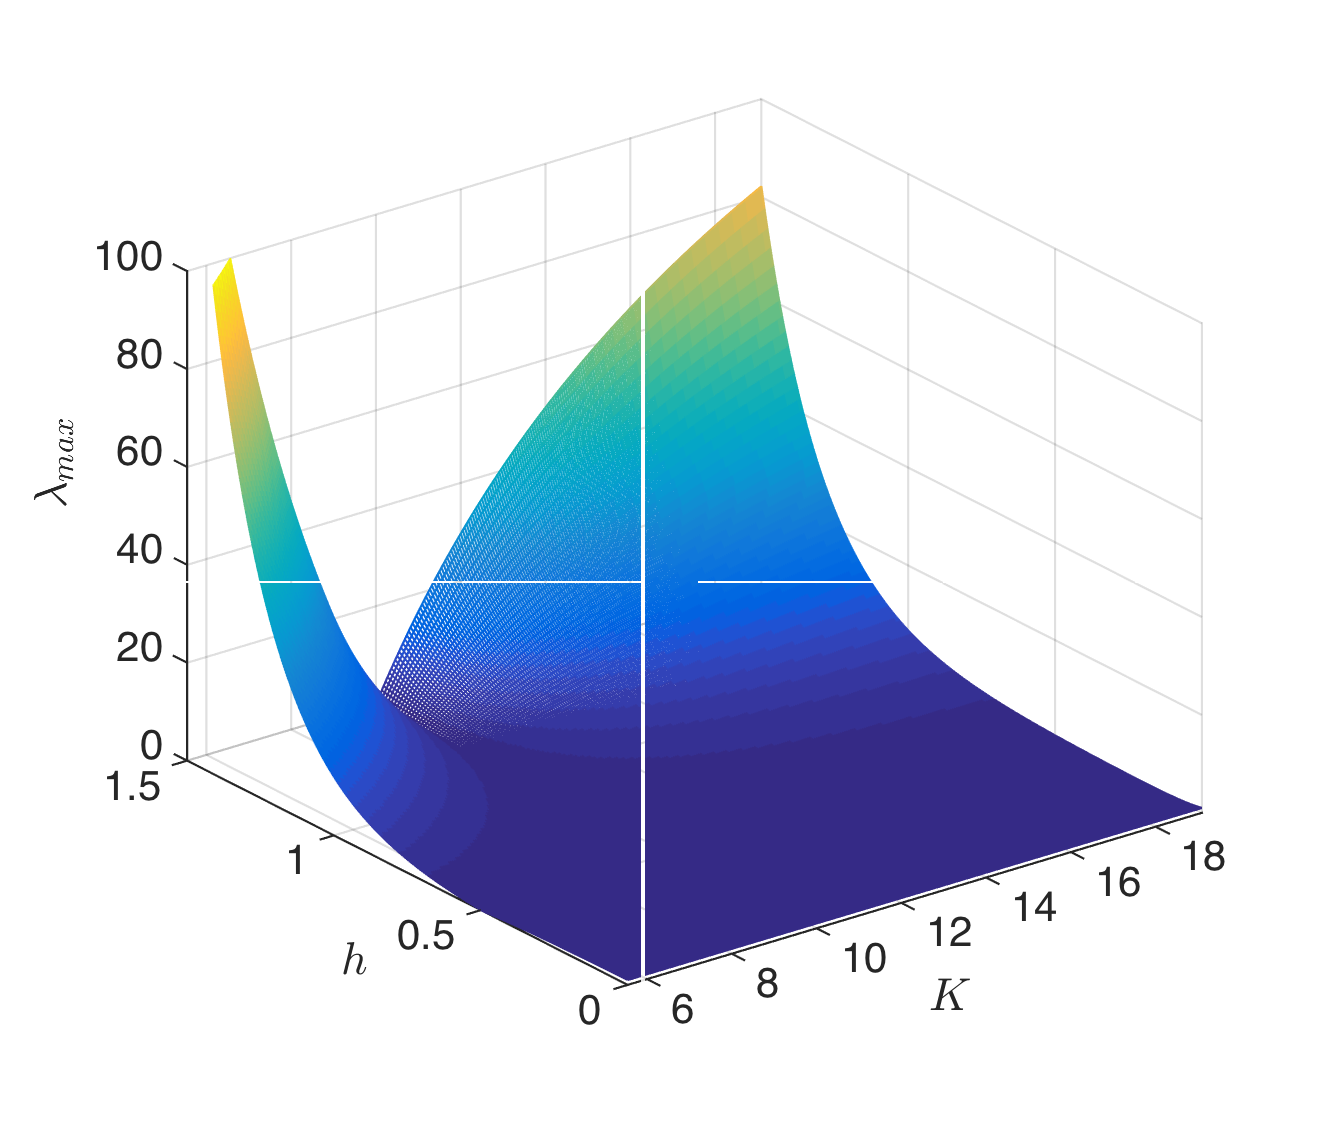
\psfig{file=3D_lambda_1D.eps,height=1.6in,width=1.8in,clip=}\hspace{-4mm}{\footnotesize (b)}}
  \caption{Plot (a): Contour plot of $\lambda_{\max}(K,h)$. The white region denotes the stable region where $\lambda_{\max}(K,h) < 1$ and the green region denotes the unstable region where $\lambda_{\max}(K,h) > 1$. Plot (b): Geometric shape of $\lambda_{\max}(K,h)$.}\label{fig:SISO_contour}
\end{figure}

After characterizing the relationship between the maximum allowable update period $H_{\max}$ and the controller gain $K$, the left column of Fig.\ref{fig:SISO_performance} compares the system performances following the controller design and implementation algorithm when the penalty coefficient $W_h$ on communication varies. The penalties on state and input are fixed at $W_x = 1$ and $W_u = 1$. Recall that operations at the maximum allowable update period $H_{\max}$ would lead to undesired oscillatory responses. To smoothen the closed-loop responses, we introduce a coeffecient $\epsilon$ so that the actual update period in operation is $h = \epsilon H_{\max}$. The optimizaiton horizon is chosen as $H = 6$, which ensures that $H > \epsilon H_{\max}$ for any $K$ in consideration, namely at least one update period is contained in the optimization horizon.

\begin{figure}[hptb]
  \centerline{\hspace{2mm}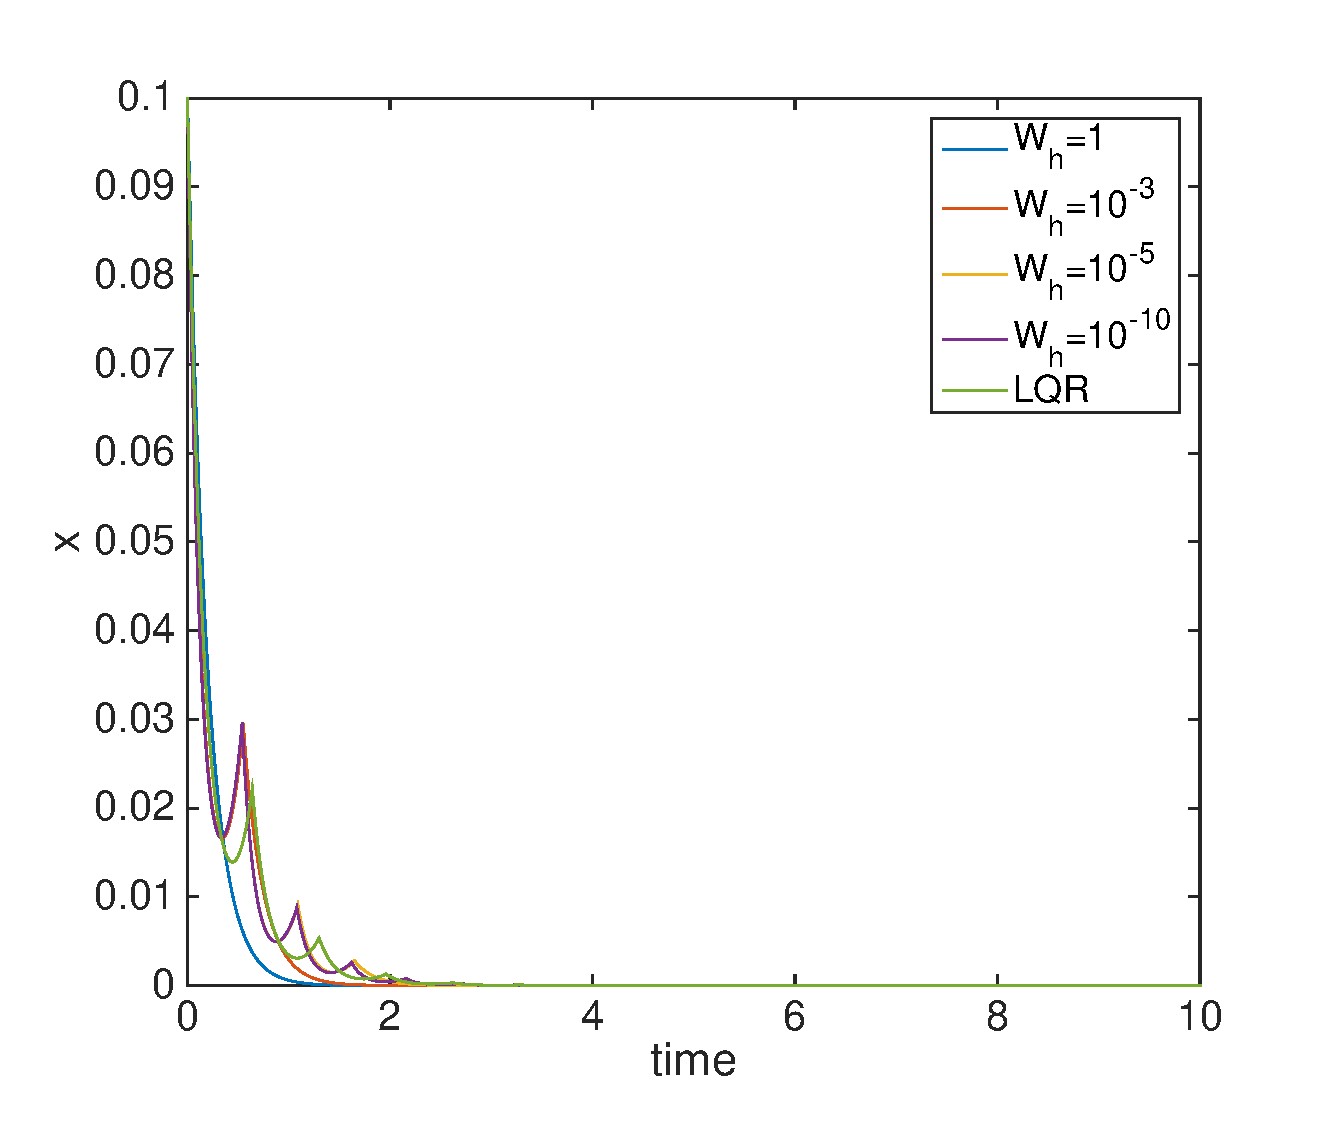
\psfig{file=x_Wh.eps,height=1.6in,width=1.8in,clip=}\hspace{-4mm}{\footnotesize (a)}
  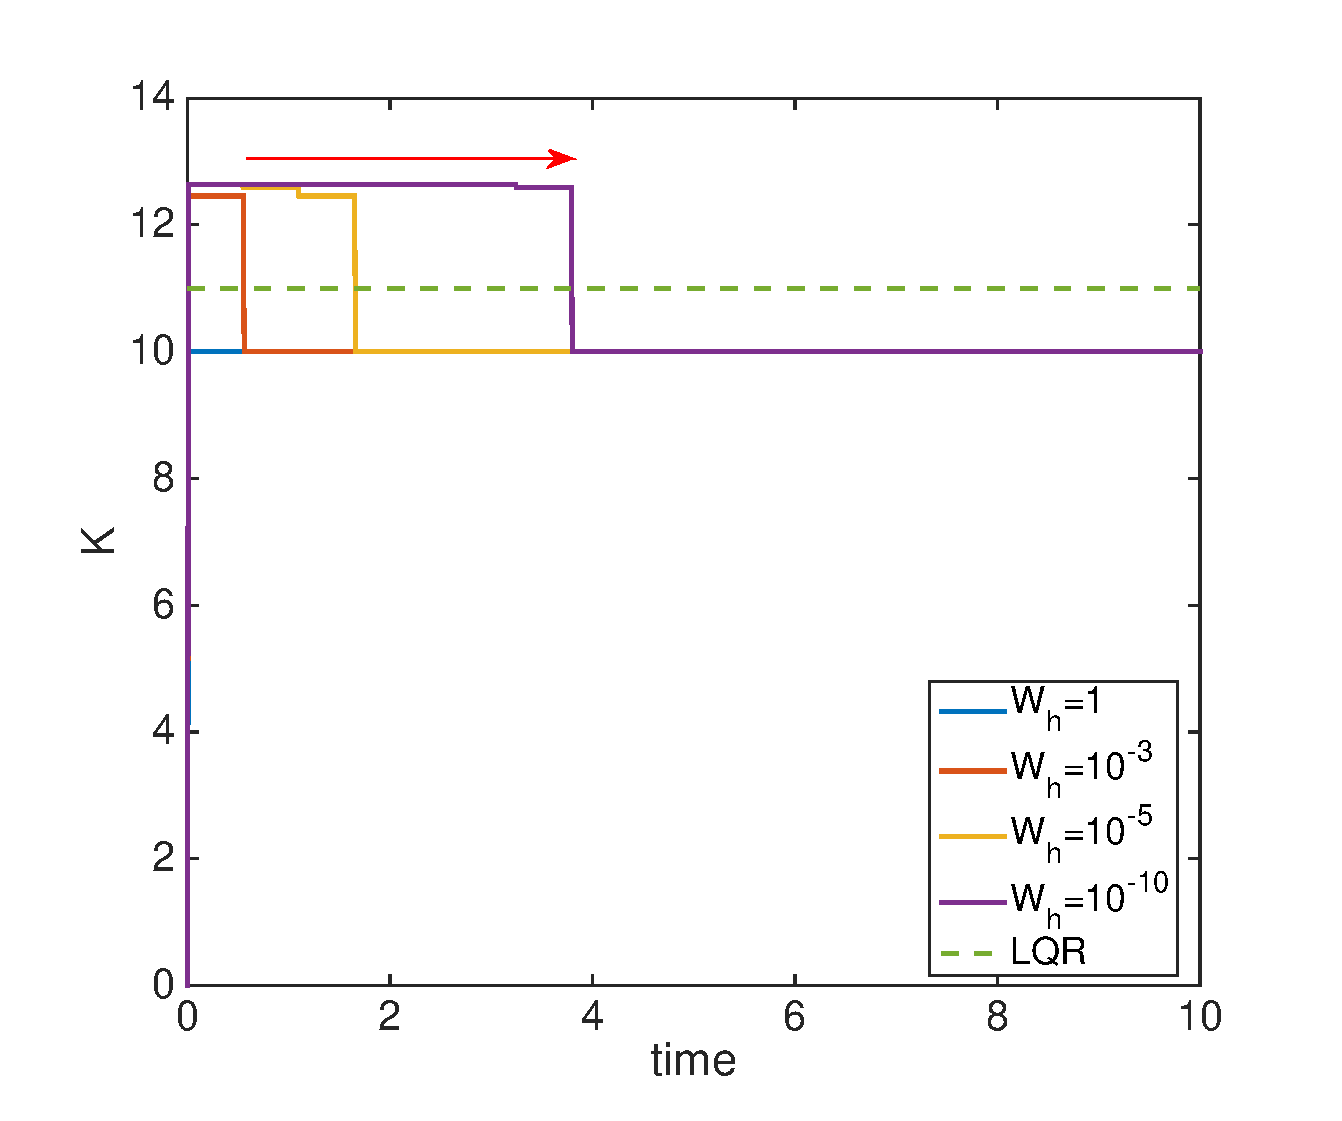
\psfig{file=K_Wh.eps,height=1.6in,width=1.8in,clip=}\hspace{-4mm}{\footnotesize (b)}}
  \centerline{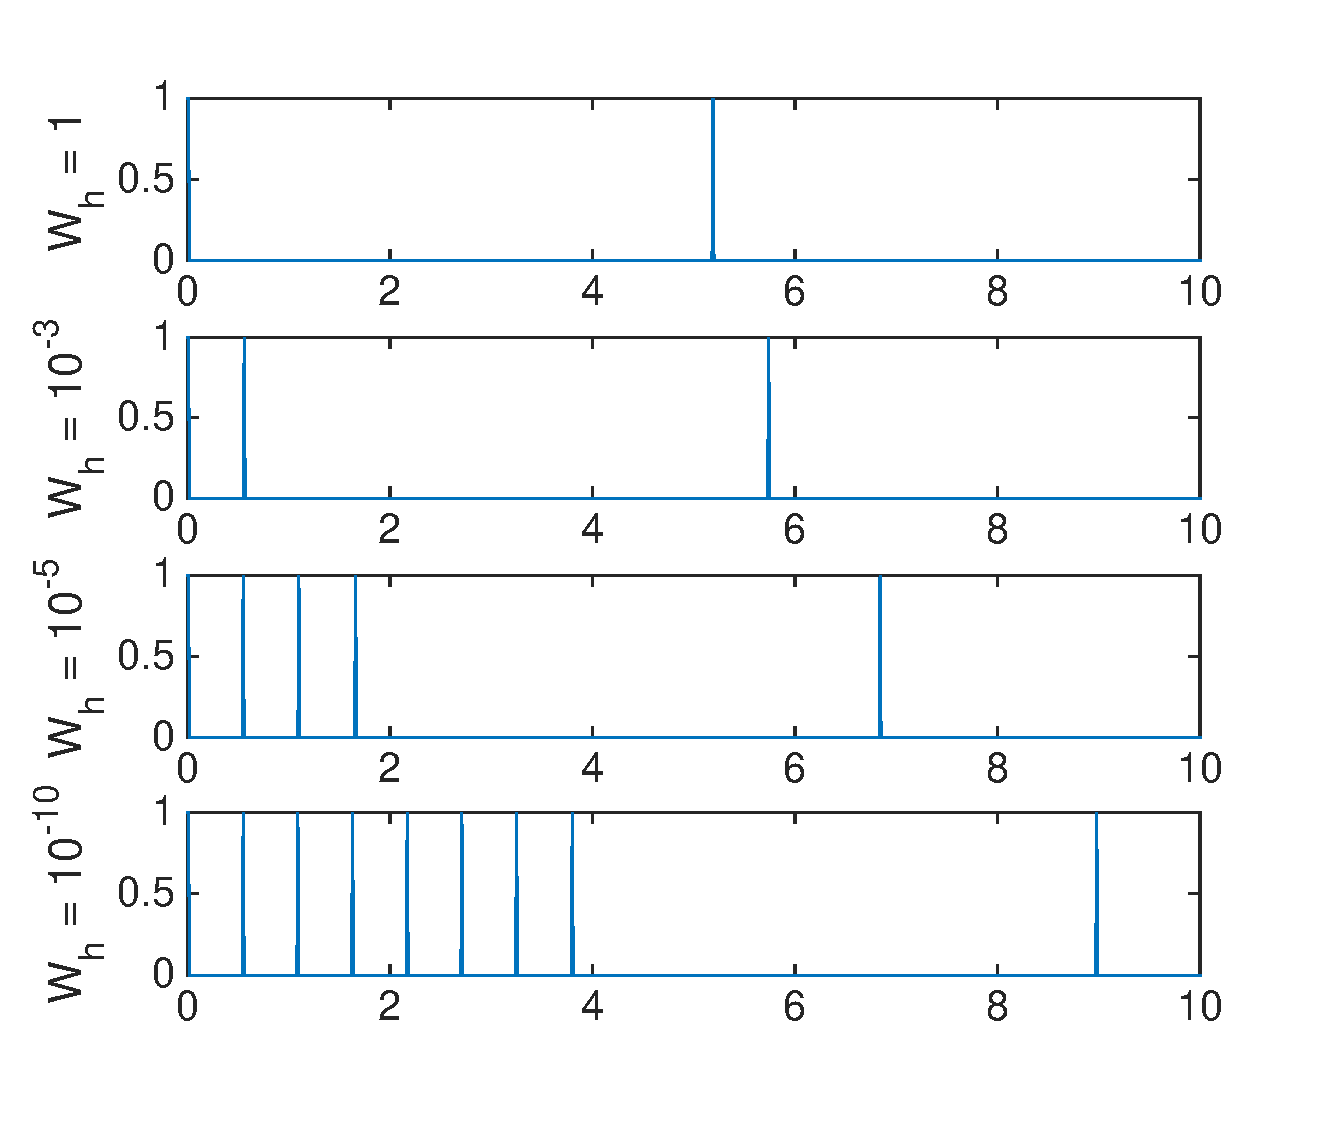
\psfig{file=update_Wh.eps,height=1.6in,width=1.8in,clip=}\hspace{-4mm}{\footnotesize (c)}}
  \caption{Performance comparisons of: (a) the closed-loop state profile, (b) the controller gain $K$, and (c) the model update frequencies when the weighting parameter $W_h$ changes.}\label{fig:SISO_performance}
\end{figure}

The lines corresponding to different $W_h$ in Fig.\ref{fig:SISO_performance} (a) show similar closed-loop state profiles. The impact of penalty on communication can be observed clearly from Fig.\ref{fig:SISO_performance} (b) and (c). When $W_h = 1$ (depicted by the blue lines in Fig.\ref{fig:SISO_performance} (b) and first subplot in (c)), as the controller penalizes heavily on communication so that the controller gain starts and maintains constant at $K = 10$ where $H_{\max}$ reaches its maximum referring to Fig.\ref{fig:SISO_contour}, and the resulting model update frequency is the lowest among the four scenarios. As $W_h = 1$ decreases, the relative penalties on the state and input increase, leading to a more aggressive controller and increased network utilization.





\subsection{CSTR example}\label{sec:CSTREx}
In this section, we illustrate some implementation issues of the optimization-based controller using a chemical process example involving a non-isothermal continuous-stirred tank reactor. The process dynamic model (\cite{christofides2005control}) is given by:

\begin{equation}
  \begin{aligned}
    \frac{dC_A}{dt} &= \frac{F}{V}(C_{A0} - C_A) - k_0\exp\left(\frac{-E}{RT}\right)C_A\\
    \frac{dT}{dt} &= \frac{F}{V}(T_{0} - T) + \frac{-\Delta H}{\rho_m c_p}k_0\exp\left(\frac{-E}{RT}\right)C_A + \frac{Q}{\rho_m c_p V}
  \end{aligned}
\end{equation}

where $C_A$, $T$, and $V$ denote the concentration of $A$, the reactor temperature, and the reactor volume, respectively. $C_{A0}$ and $T_{0}$ denote the concentration of $A$ and the temperature of the inlet stream, respectively. $Q$ denotes the rate of heat input to the reactor which is taken as the manipulated input. $\Delta H$, $k_0$, and $E$ denote the enthalpy, pre-exponential constants and activation energy, respectively, of the first-order elementary reaction $A \rightarrow P$, $c_p$ and $\rho_m$ denote the heat capacity and density of fluid in the reactor. Using typical values for the process parameters (see \cite{christofides2005control}), the process has an open-loop unstable steady state at $(C_{A}^s, T^s) = (0.575 mol/L,\ 395.05 K)$. The control objective is to stabilize the process near this steady state using minimum sensor-controller communication. Linearizing the system at the unstable equilibrium point yields the following parameters for the system described in the form of Eq.\ref{eqn:PlantState}
\begin{equation}
    A = \left[\begin{array}{cc}
        -1.74   & -0.03\\
        147.97  & 4.45
      \end{array}\right],\
    B = \left[\begin{array}{c} 0 \\ 0.0042 \end{array}\right]
\end{equation}
where $A$ has two eigenvalues at $\lambda_1(A) = 3.71$ and $\lambda_2(A) = -1.0$, respectively. Approximate model parameters and model uncertainties are
\begin{equation}\label{eqn:ModelPara}
  \begin{array}{ll}
  \widehat{A} = \left[\begin{array}{cc}
      -1.8  & 0\\
      150   & 5
    \end{array}\right] &
  \widehat{B} = \left[\begin{array}{c} 0 \\ 0.005 \end{array}\right]\\
  \delta_A = \left[\begin{array}{cc}
      0.06    & -0.03\\
      -2.03   & -0.55
    \end{array}\right] &
  \delta_B = \left[\begin{array}{c} 0 \\ 0.0008 \end{array}\right]
  \end{array}
\end{equation}

From stability condition, we can again generate a contour plot of $\lambda_{\max}(K,h)$ and determine the adimissible range of $h$ that renders closed-loop stability. Notice that as the system is 2-dimensional, the feedback gain is made up of two elements, $K = [k_1\ k_2]$. To simplify the illustration, we first fix $k_2 = 2000$ and generate a contour plot of $\lambda_{\max}(h,k_1)$. Similar contour plot of $\lambda_{\max}(h,k_2)$ when fixing $k_1$ can be generated in the same way. Figures of $\lambda_{\max}(h,k_2)$ are omitted here.

\begin{figure}[hptb]
  \centerline{\hspace{2mm}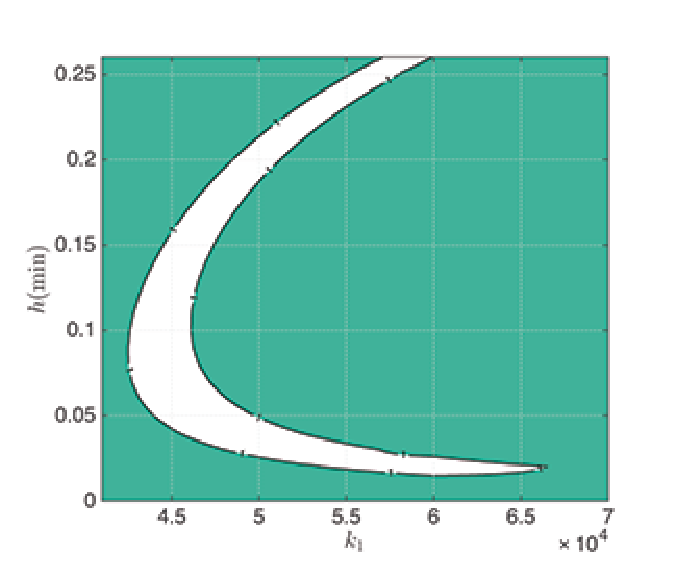
\psfig{file=Contour_lambda1.eps,height=1.6in,width=1.8in,clip=}\hspace{-4mm}{\footnotesize (a)}
  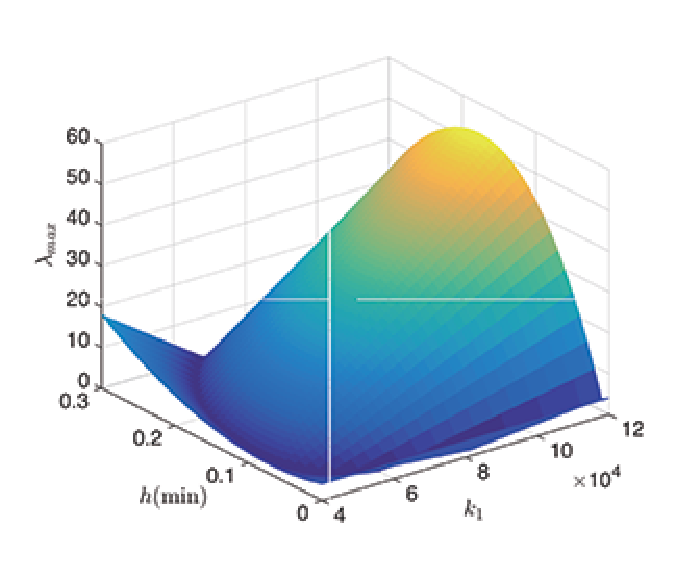
\psfig{file=3D_lambda.eps,height=1.6in,width=1.8in,clip=}\hspace{-4mm}{\footnotesize (b)}}
  \caption{Plot (a): Contour plot of $\lambda_{\max}(h,k_1)$. The white region denotes the stable region where $\lambda_{\max}(h,k_1) < 1$ and the green region denotes the unstable region where $\lambda_{\max}(h,k_1) > 1$. Plot (b): Geometric shape of $\lambda_{\max}(h,k_1)$.}\label{fig:CSTR_contour}
\end{figure}

Similar to Fig.\ref{fig:SISO_contour}, Fig.\ref{fig:CSTR_contour}(a) shows $\lambda_{\max}(h,k_1)$ and is divided into two regions. The crescent-shape white region is the stable region where $\lambda_{\max}(h,k_1) < 1$, and the green outer region is the unstable region where $\lambda_{\max}(h,k_1) > 1$. Again, the contour line of $\lambda_{\max}(h,k_1) = 1$ separates the stable and unstable regions. However, unlike Fig.\ref{fig:SISO_contour} for the SISO system where for a given feedback gain $K$ there is only an upper limit $H_{\max}$ on the update period $h$, due to the increased dimensionality, the stability region in Fig.\ref{fig:CSTR_contour}(a) is complicated (comparing the geomatric shapes depicted in Fig.\ref{fig:SISO_contour}(b) and Fig.\ref{fig:CSTR_contour}(b)) and a lower limit $H_{\min}$ on $h$ also exists. This means that for a certain controller gain $K$ the closed-loop system isstable only  if the update period takes value within a certain range, and instability could occur even if the model state is updated continuously. Take $K = [4.41\times 10^4\ 2000]$ as an example. The admissible range of the update period $h$ is the intersection of the red vertical line and the white region in Fig.\ref{fig:CSTR_contour}(a), i.e. $h\in [0.05min, 0.145min]$.

To implement the controller design method and communication strategy, it is crucial to characterize the admissible range of update period $h$. As discussed previously, the characterization can be performed off-line reducing computational expenses in system operation. Besides the maximum allowable update period $H_{\max}$ defined earlier, we introduce $H_{\min}$ as the minimum allowable update period. Notice that there is another complexity resulted from the higher dimensionality. Reffer to Fig.\ref{fig:CSTR_contour}(a), when $[k_1 \in (4.1\times 10^4, 4.6\times 10^4)$, the feasible (white) region has two branches. The existence of the disconnected sections of $h$ indicates that there are two upper and lower limit pairs of $H_{\max}$ and $H_{\min}$ for a givin controller. With the purpose of reducing network utilization, in such cases, we ignore the lower branch, and only take the upper branch to determine the corresponding $H_{\max}$ and $H_{\min}$. For this specific system, we consider the range of controller gain $k_1 \in [4.2\times 10^4, 5.0\times 10^4]$ and $k_2\in [1.4\times 10^2, 3.2\times 10^2]$ and Fig.\ref{fig:HmaxHmin}(a) and (b) show contour plot of $H_{\max}(k_1,k_2)$ and $H_{\min}(k_1,k_2)$ respectively.

\begin{figure}[hptb]
  \centerline{\hspace{2mm}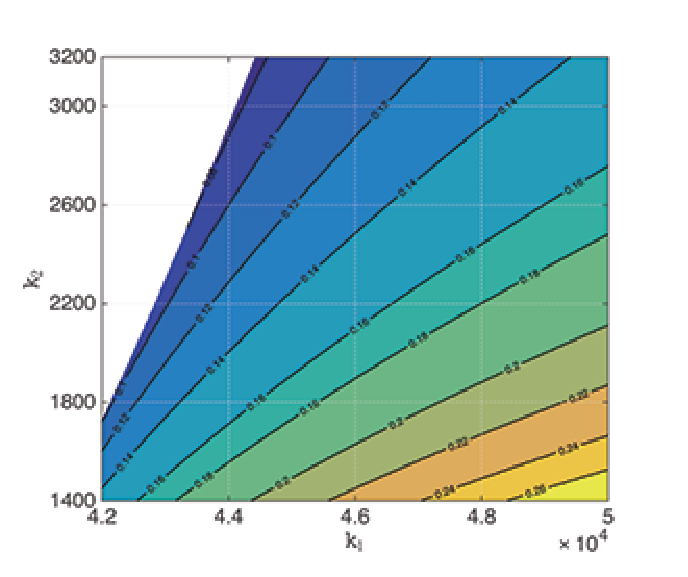
\psfig{file=0911_Hmax.eps,height=1.6in,width=1.8in,clip=}\hspace{-4mm}{\footnotesize (a)}
  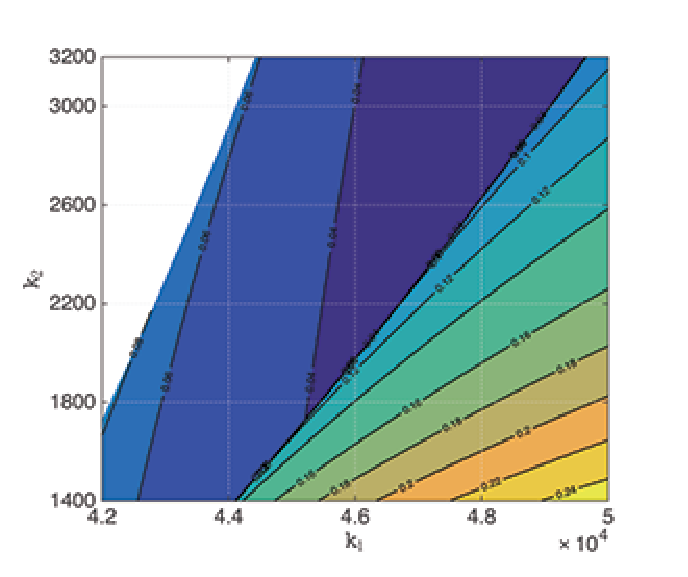
\psfig{file=0911_Hmin.eps,height=1.6in,width=1.8in,clip=}\hspace{-4mm}{\footnotesize (b)}}
  \centerline{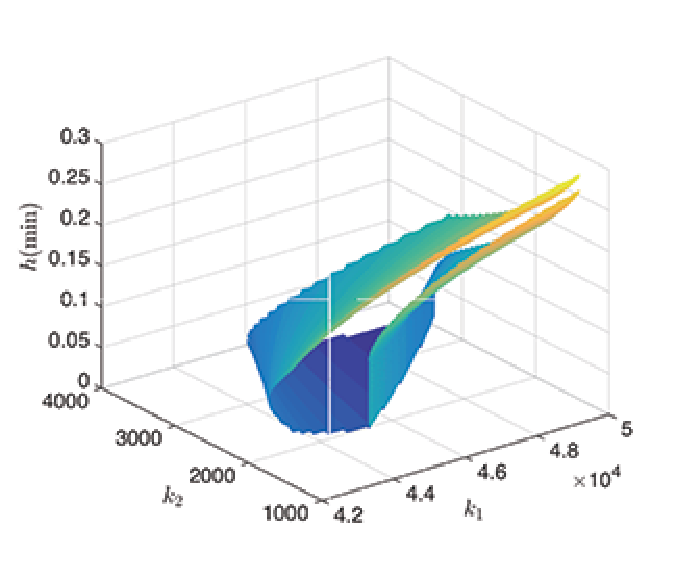
\psfig{file=0911_HmaxHmin.eps,height=2.5in,width=3in,clip=}\hspace{-4mm}{\footnotesize (c)}}
  \caption{Contour plot of (a) $H_{\max}(k_1,k_2)$ and (b) $H_{\min}(k_1,k_2)$. The white region is where solution to $H_{\max}$ or $H_{\min}$ does not exist. Plot (c): Geometric shape of the adimissible range of $h$ in the $k_1$-$k_2$ space.}
  \label{fig:HmaxHmin}
\end{figure}

Fig.\ref{fig:HmaxHmin}(c) shows geometric shape of the admissible $h$ range, which is denoted as the space wrapped by the surface of $H_{\max}$ and $H_{\min}$. For a given feedback gain $K = [k_1\ k_2]$, the update period $h$ has to take values within the wrapped space for the closed-loop system to be stable. Notice that there is a stair up at the right corner. This is due to the existence of multiple branches of $h$ exist and that only the upper branch is considered for operational benefit. Plots in Fig.\ref{fig:HmaxHmin} do not have to be generated to determine the allowable model update period range, but they can help to visualize the general trend of $H_{\max}$ and $H_{\min}$ in relationship with the controller gain. Recall that response of the closed-loop system would be oscillatory when the model update period is exact at $H_{\max}$ or $H_{\min}$, the actual update period is selected as
\begin{equation}\label{eqn:hact}
  h = H_{\min} + \epsilon(H_{\max} - H_{\max})
\end{equation}
where $\epsilon$ is a tunable parameter that can take values between 0 and 1. $\epsilon = 0.7$ in this simulation study. After characterizing the relationship between the controller gain $K$ and its corresponding update period, the optimization-based controller is ready to be implemented. To better demonstrate the adaptive nature of the optimal controller, we compare it with a linear quadratic regulator (LQR) subject to the same panalty coefficients $W_x = 1$ and $W_u = 1$. The LQR determines the state-feedback gain $K^{LQR}$ by minimizing the cost function of
\begin{equation}
  J = \int_0^\infty (x^TW_xx + u^TW_uu)dt
\end{equation}
and the state-feedback gain is computed to be $K^{LQR} = [4.1\times 10^4\ 2\times 10^3]$ using the model parameters in Eq.\ref{eqn:ModelPara} and the panalty coefficients $W_x = 1$ and $W_u = 1$. The upper and lower limits on the model update period for the LQR can be determined from Fig.\ref{fig:HmaxHmin}, and the results are $H_{\max}^{LQR} = 0.15min$ and $H_{\max}^{LQR} = 0.05min$. The actual model update period is therefore $0.05 + 0.7\times(0.15 - 0.05) = 0.12$ according to Eq.\ref{eqn:hact}. Fig.\ref{fig:CSTRPerformance} show a comparison of the the system performances under the optimization-based controller (referred to as "optimal" in the figures and are denoted by the blue lines) and the LQR (denoted in red).

\begin{figure}[hptb]
  \centerline{\hspace{2mm}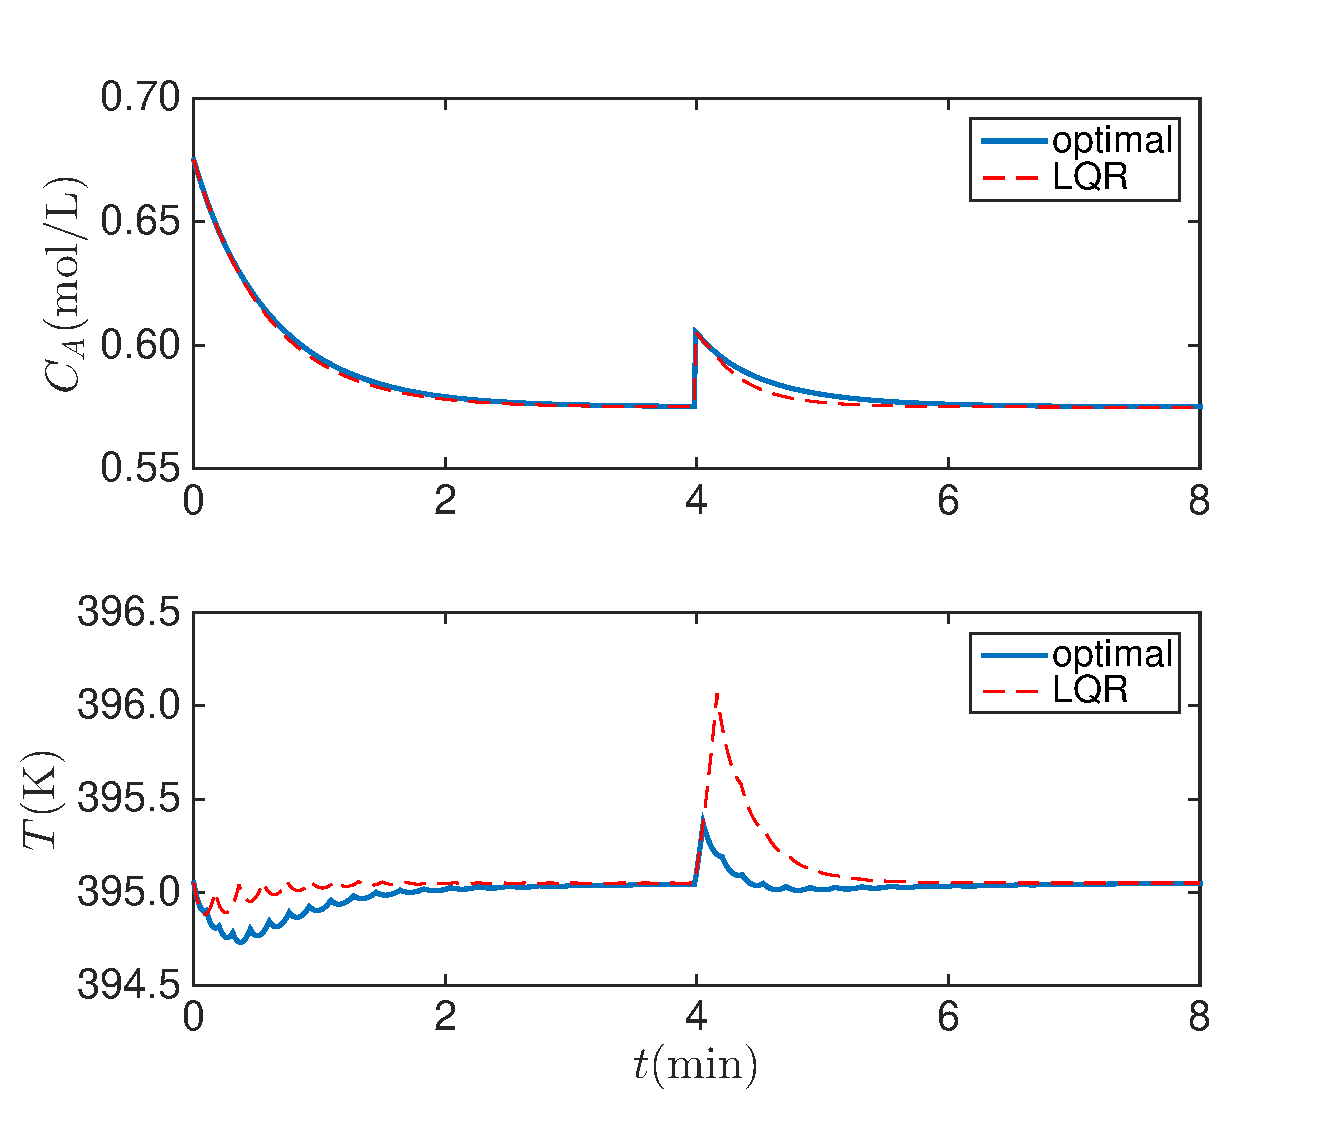
\psfig{file=0911CSTR_state_t8.eps,height=1.6in,width=1.8in,clip=}\hspace{-4mm}{\footnotesize (a)}
  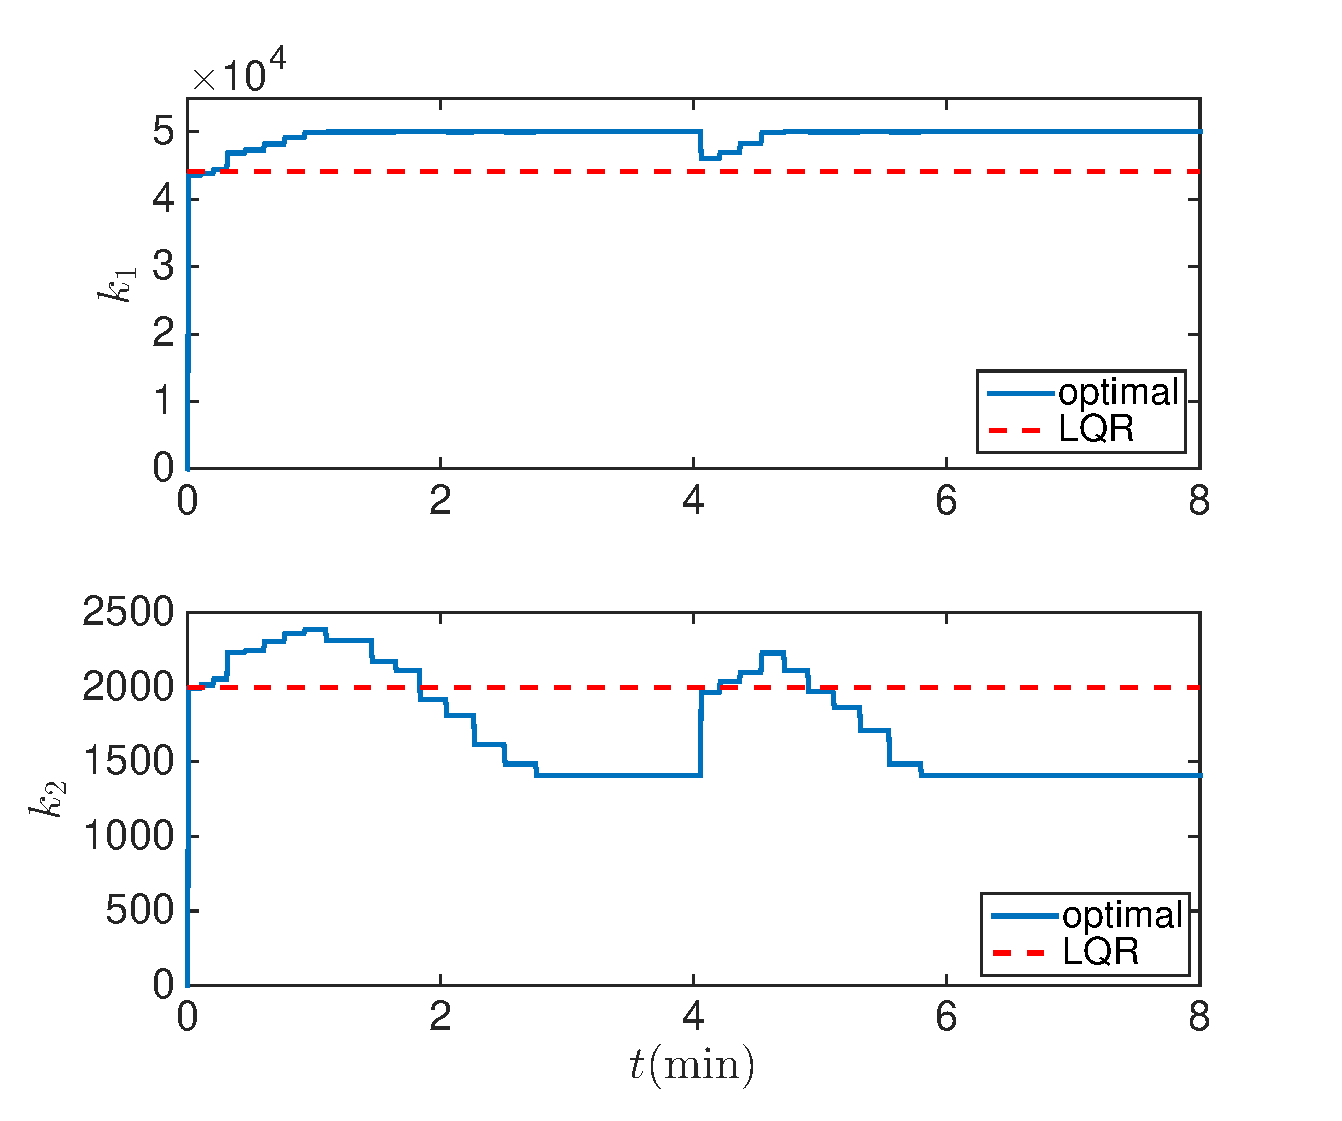
\psfig{file=0911CSTR_K_t8.eps,height=1.6in,width=1.8in,clip=}\hspace{-4mm}{\footnotesize (b)}}
  \centerline{\hspace{2mm}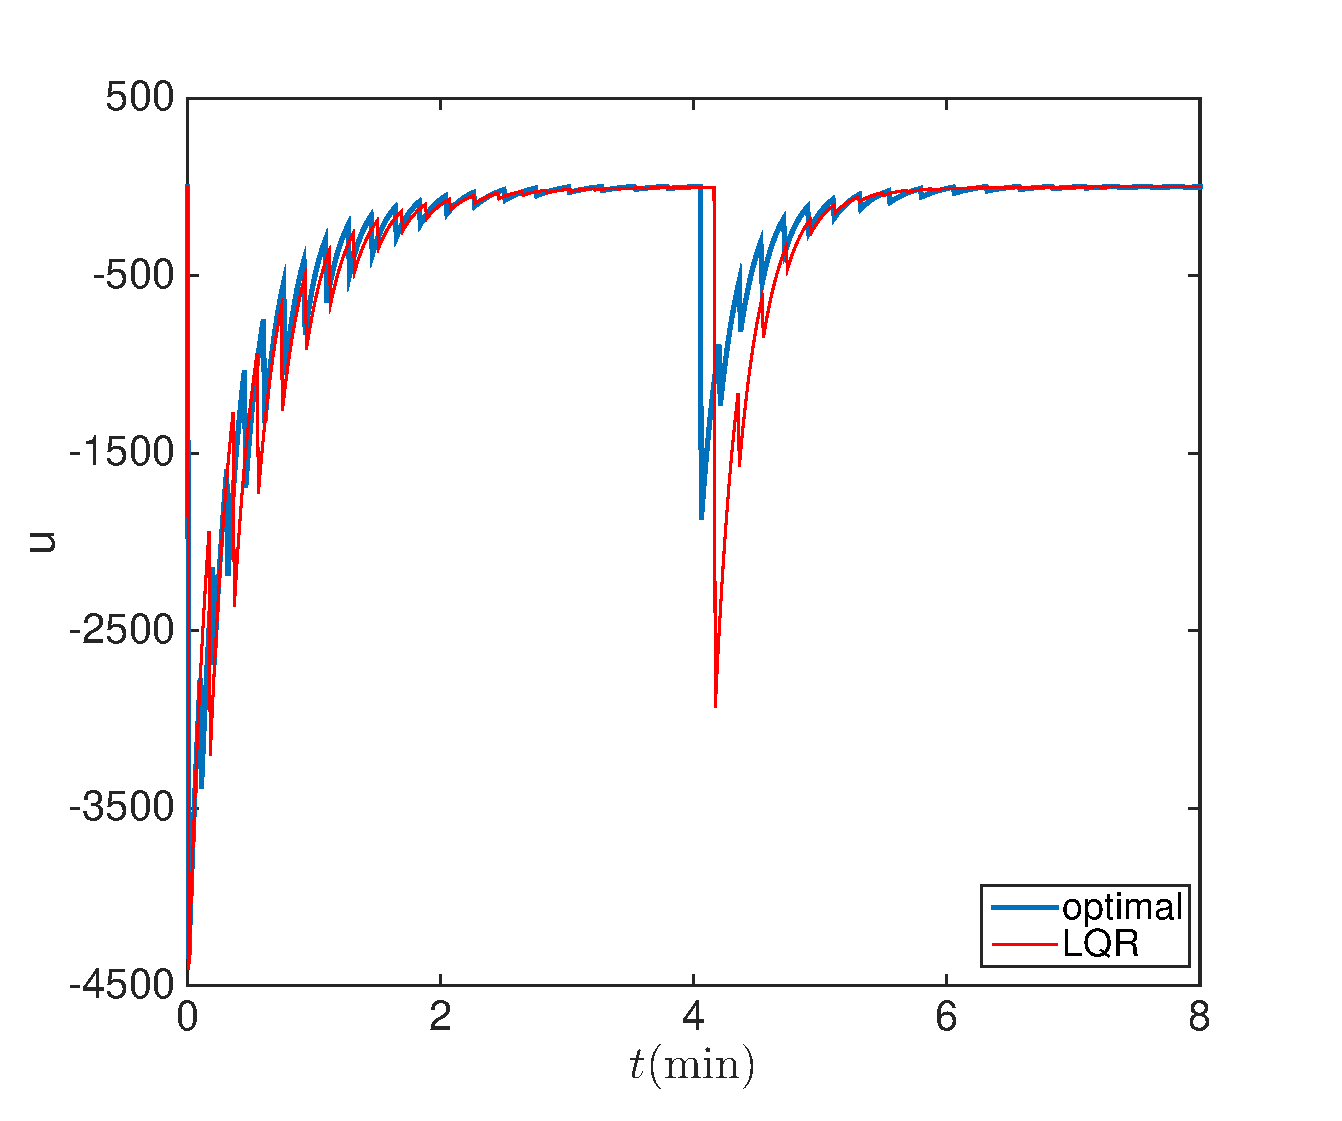
\psfig{file=0911CSTR_u_t8.eps,height=1.25in,width=1.8in,clip=}\hspace{-4mm}{\footnotesize (c)}
  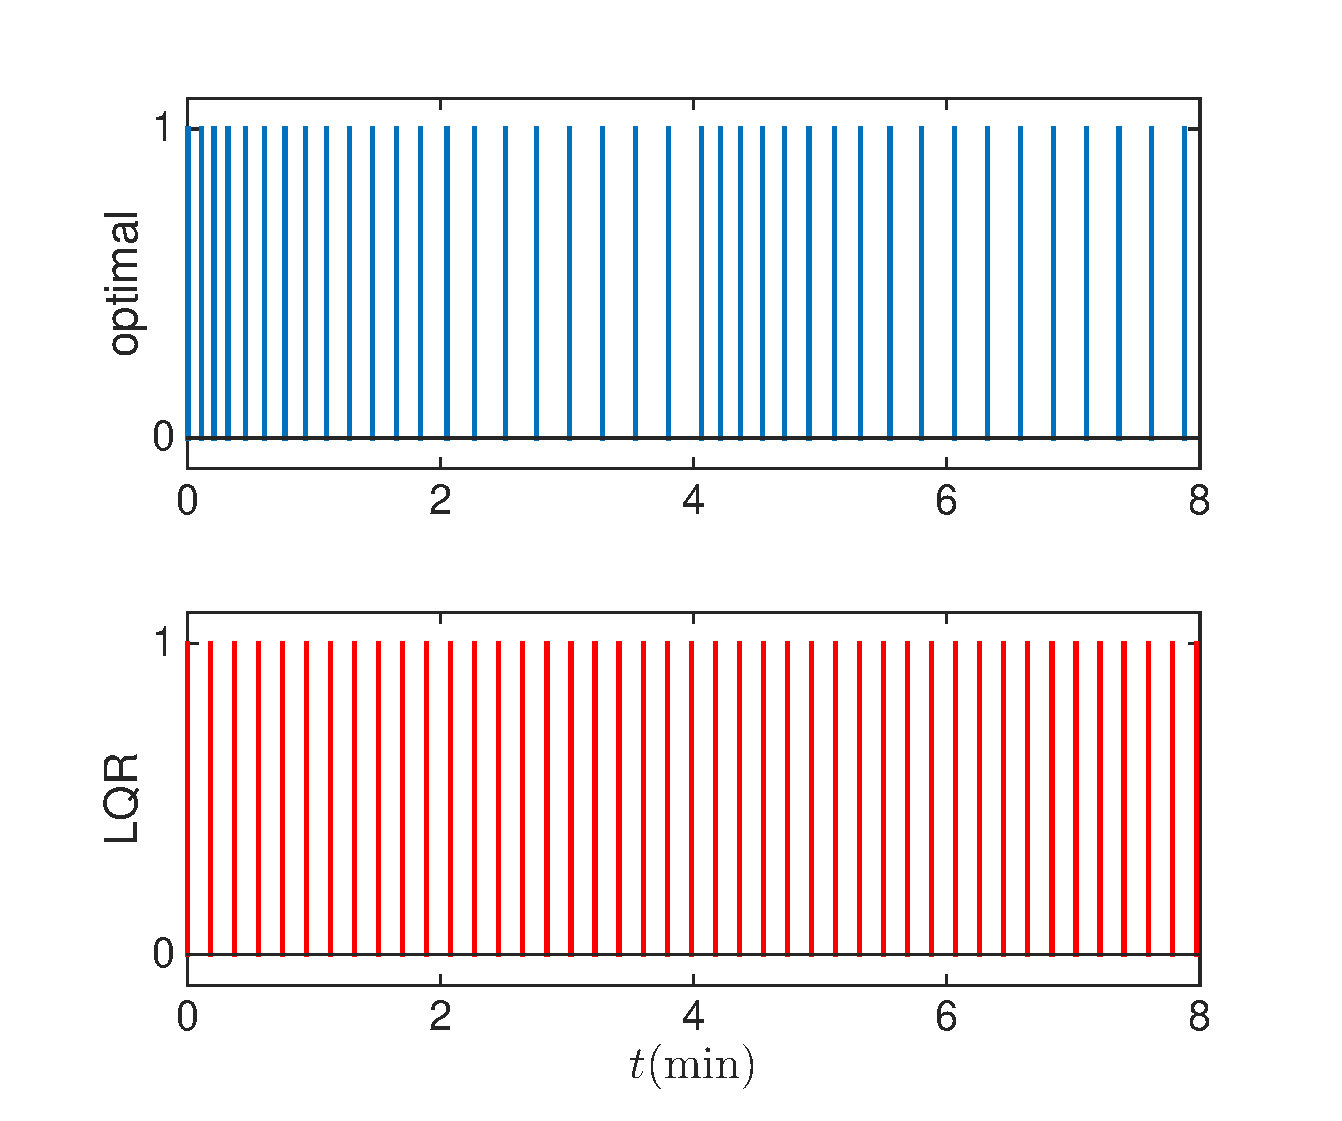
\psfig{file=0911CSTR_update_t8.eps,height=1.6in,width=1.8in,clip=}\hspace{-4mm}{\footnotesize (d)}}
  \centerline{\hspace{2mm}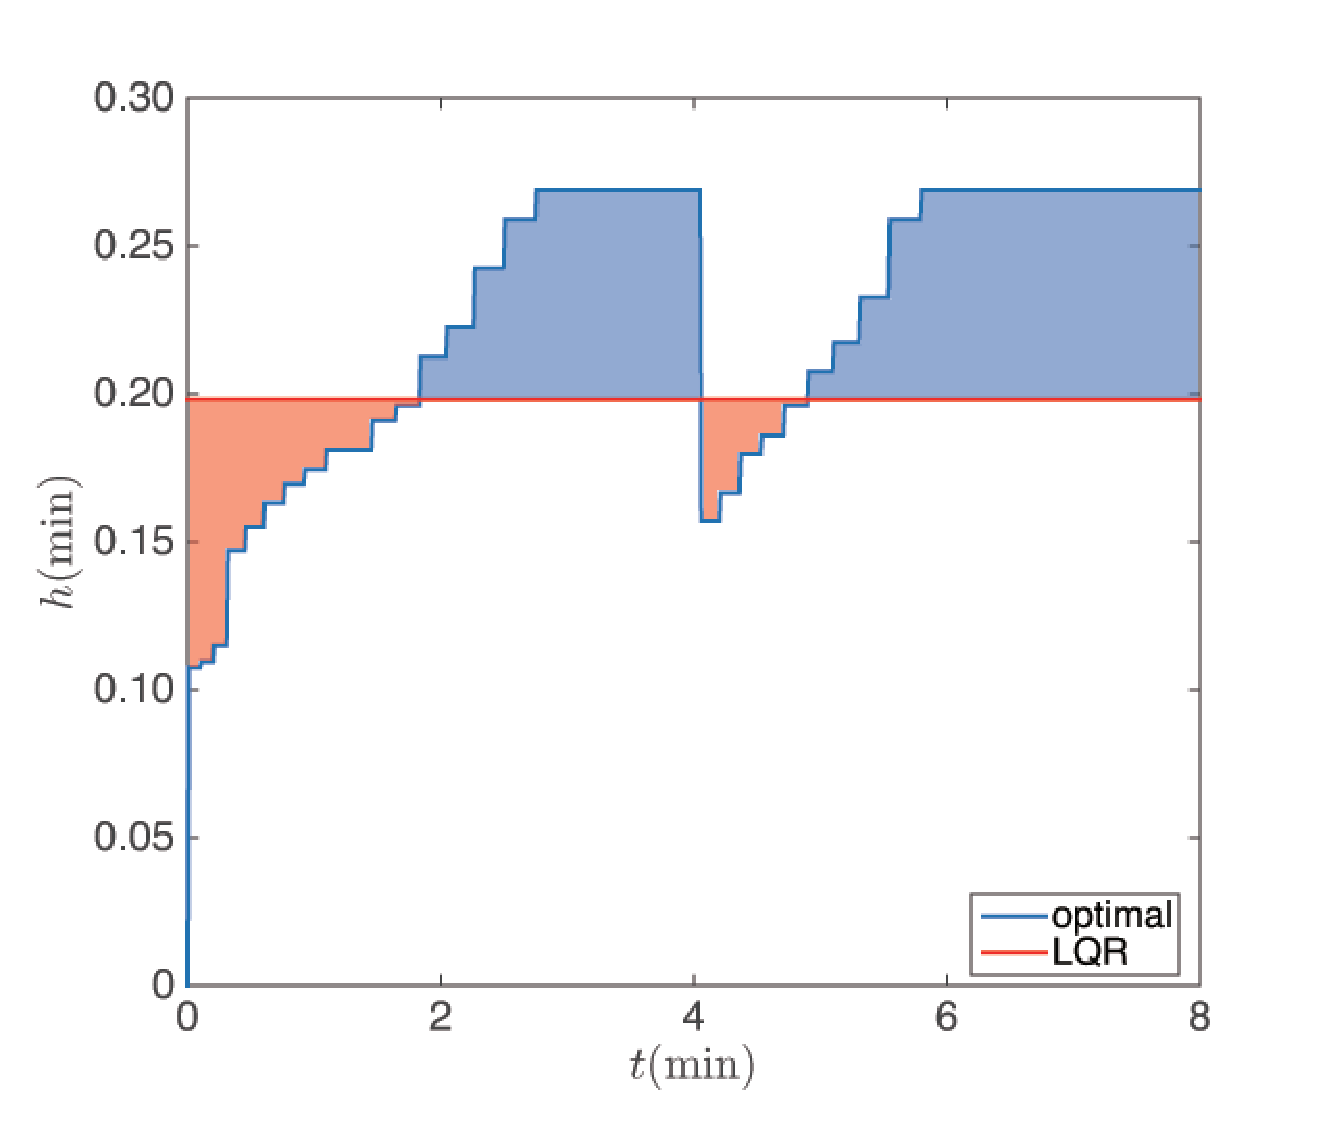
\psfig{file=0911CSTR_h.eps,height=1.25in,width=1.8in,clip=}\hspace{-4mm}{\footnotesize (e)}}
  \caption{Plot (a): Closed-loop state profiles. Plot (b)-(c): Profiles of the controller gain and manipulated input. Plot (d): Comparison on model update frequencies under the optimal controller and the LQR. Plot (e): Comparison on network utilization. }\label{fig:CSTRPerformance}
\end{figure}

An impulse disturbance is introduced at $t = 4min$ to test robustness of the controllers. Fig.\ref{fig:CSTRPerformance}(a) shows comparable state convergence rate during the transient period $t \in [0,2]min$, but the optimal controller performs better under disturbances. This is because the optimization-based controller is able to suppress the influence of the unexpected disturbance by increasing the controller (see Fig.\ref{fig:CSTRPerformance}(b) and (c)) and compromising the communication load (see Fig.\ref{fig:CSTRPerformance}(d)) in drive the state back to equilibrium faster. The comparison with the LQR clearly shows that the design and implementation methodology ensures that the optimal controller is able to adjust its control parameters to adaptive to changes in operating conditions spontaneously. The udpate profile Fig.\ref{fig:CSTRPerformance}(d) and the actual model udpate period profile Fig.\ref{fig:CSTRPerformance}(e) compare network utilization for the two controllers. The spikes in Fig.\ref{fig:CSTRPerformance}(d) correspond to the time instances of model update or measurement transimission in each simulation. Apparently the LQR relys on a constant update period, while the optimal controller adjusts its model update period according to the real-time optimization solution implied by the change of density of the blue spikes. A more quantative measure of the network utilization is the actual model udpate period profile Fig.\ref{fig:CSTRPerformance}(e) which shows the model update period implemented at a given time. For the purpose of reducing network utilization, it is preferred that the area under the curve to be as large as possible. This is another way of measuring the network load. The area under the $h$ curve is determined by the decision of un update period at a update time $t_k$ and how long it is implemented $(t_{k+1} - t_k)$. Mathematically, the area is defined as

\begin{equation}
	Area = \sum_{k=1}^\infty h_k^2
\end{equation}

Even though the optimal controller relies on shorter model update period during the transient period and when the system is perturbed with disturbances, it is able to maintain a relatively long update period during regular operation (when the state is close enought to its steady state). The reduction on network utilization would be even more significent for longer operations.




\bibliographystyle{IEEEtran}
\bibliography{2017ACC_opt}

\end{document}
